\chapter{Background}
\label{cha:background}

This section presents all the background information relevant to the thesis, that
are required in order to properly understand the matter of the project, the
problem, the technologies and the solution.

We start in \cref{cha:CPU speculation contract} by explaining what a CPU speculation
contract is, and why it is important for the scope of this thesis. Then we then move
to \cref{cha:Revizor}, where we discuss about the Revizor tool, that is used in the
research project to detect the contract of a CPU. We detail how it works and
some background information. In \cref{cha:Rosette}, we talk about Rosette, the solver-aided
programming language that we used to encode the violations reported from Revizor.
With this tool we are able to feed the loop, that is the base of this project.
In \cref{cha: Loop outlook}, we present an overview of the loop that is used to synthesize
the CPU contract, using all the tools and language discussed in previous
sections, and therefore deeper explaining the research project this thesis is part
of. In \cref{cha:DSL}, we discuss about the Domain Specific Language (DSL) that the
team used before this thesis's project, and why it was not enough for the scope
of the overall project. In \cref{cha:BIR}, we talk about the Binary Intermediate
Representation (BIR) language, that has been chosen to replace the DSL. Also, in
\cref{cha:Language comparison} there is a more in-depth comparison and explanation
of the differences between the two languages, with a brief about why BIR showed
to be the best choice for this project and this whole domain.

\section{CPU speculation contract}
\label{cha:CPU speculation contract} Before diving into what a CPU speculation
contract is, it is better to have a clear idea of what speculative execution is.
In speculative execution, the CPU tries to predict the path of a branch operation
before the actual path to follow is known. This is done to increase a processor's
performance, as the CPU can execute instructions beforehand, concurrently. Once the
actual path is known, the CPU can discard or confirm the speculative execution.

\begin{figure}
  \centering
  \begin{varwidth}
    {\linewidth} \begin{verbatim}
      if (x == 1) {
        y = 1;
      } else {
        y = 2;
      }
          \end{verbatim}
  \end{varwidth}
  \label{fig:snip1}
  \caption{Conditional statement}
\end{figure}

For example, consider the snippet in \cref{fig:snip1}. The CPU can predict that the
path is the one on the true branch (hence, y=1), and starting to execute the code
in there. At the same time, the CPU has to check if the condition holds,
evaluating the predicate. If the evaluation confirms that the speculation was right,
the CPU can confirm the speculative execution, and continue with the execution.
Otherwise, it discards the execution and run the real path. This usage of
concurrent execution allows the performance increase, since if the speculation turned
out to be right, then there are less cycle to be made in the future, while if that
was not the case, the CPU is at the same point as if the speculation would have
never been made.

CPU vendors started to use this approach to increase the performance of their
modules once the refresh rate reached a plateau around 4GHz, and the transistor's
size was not decreasing anymore, due to the physical limits of the materials. So,
to get faster hardware they decided to invest in speculative execution. This gave
room for improvements, but also to some vulnerabilities, such as Spectre \cite{spectreattack},
Meltdown \cite{meltdownattack}, Riddle \cite{ridl}, Fallout \cite{fallout}, LVI \cite{lvi}
and so on. This are the kinds of vulnerabilities that Revizor \cite{article} (\cref{cha:Revizor})
tries to detect. This vulnerabilities are one of the reason this project exists,
since the synthesis of contract would be the first step to find vulnerable code,
and then eventually patch it. This could be future work for the project, as also
discussed in \cref{cha:Future work}.

With this in mind, the speculation contract of a CPU can be seen as an agreement
or policy that governs the behavior of the speculative execution. A contract is usually
formed by different so-called constraints, that are all the rules that the CPU
has to follow in order to be compliant with the contract. All constrains are usually
encoded with the machine-specific code of the CPU, that is not accessible from
the users. This is why we ofter refer to this contract as a black-box contract,
and that is why this project aims to synthesize them.

One of the main goals of this project is synthesizing this contract, using all the
tools that follows in the next sections, and then represent them in a human-readable,
standard language. This language, at the beginning was a DSL, \cref{cha:DSL}, but
in this thesis project, we replace it with BIR, \cref{cha:BIR}.

\section{Revizor}
\label{cha:Revizor} Revizor is an open source fuzzing tool developed by a Microsoft
Research team \cite{article}. It has been developed to detect black-box CPU
informational leakages, just starting from a CPU speculation contract. Then, it generates
a number of test cases, executing therefore some fuzzing to detect eventual
leakages in the contract. The test case is represented by a semi-random assembly
file filled with branch operations and memory accesses. Given the fact that the
assembly is known, the final state of the CPU, giving the initial state, should also
be known. But given non-predictable behaviors, such as speculative execution,
the final state can diverge from the expected one. This is when Revizor detects a
leakage of information from the CPU.

Microsoft researchers tested Revizor on different x86 Intel CPUs, finding some
known vulnerabilities, such as Spectre, MDS (Micro-architectural Data Sampling)
and LVI (Load value injection), and some novel ones. All this is done in a short
amount of time, in an automated fashion. The tool is mainly written in Python, with
some C code for performance improvements. It is available on GitHub \cite{repo},
and can be used by anyone to test any CPU. The documentation of Revizor is full
of examples and tests made \cite{misc}, along with explanation videos and conference's
recordings.

In this project, the researchers leverages Revizor as part of the tool chain (this
project starts effectively as a fork from the main Revizor code), to detect the contract
of a CPU, making therefore a step further. Starting from our current CPU speculative
contract, we run Revizor on this specification, and then we check if we obtain some
violations. If so, we infer from the violations registered the constrains of the
speculative contract of the CPU, and we enrich it with these new information. And
then we loop over. The loop is further discussed in Section
\cref{cha: Loop outlook}, when we have also further details about Rosette, that
we discuss in next section.

\section{Rosette}
\label{cha:Rosette} Rosette \cite{ros} is an open-source, solver-aided programming
language, is Racket-based and allows to write programs that are able to generate
and solve constraints. So, it takes care of verifying and synthesizing programs,
making easier to build Domain Specific Languages, doing the heavy lifting on its
own, making easier for the user to write the code.

This is not a language that is common to see, since it is mainly used in
research fields, especially when dealing with compilation, verification, computation
and solving engine. The most famous use cases and applications of Rosette are, as
right now, Jitterbug \cite{jit}, that is a framework to build and verify Just In
Time (JIT) compilers, and Serval \cite{ser}, a framework to develop automated verifiers
for system software. More applications using Rosette can be found on the site of
the project \cite{ros}. Note that these are just the open source projects that are
using Rosette.

In the project, Rosette is used to generate new constrains to the CPU contract, inferring
from the violations reported from Revizor in \cref{cha:Revizor}. This to
continue iterating over the loop until the contract is stable. It has been chosen
as it makes the development of the tools needed to handle, verify and synthesize
the contracts easier, faster and more reliable. Also, Rosette is one of the most
used and known tools in this field, so it is well documented, and further and future
development can be done by other members of the research community, that is the
main audience of the project.

\section{Loop outlook}
\label{cha: Loop outlook} The project works by iterating a loop for synthesizing
the CPU contract. The loop can be visualized in \cref{loop}. This chapter gives
an overview of the loop, the steps it takes and the stop conditions.

At the beginning, we start with a bootstrapped CPU with an initial contract, being
empty. At this point, we pass it through Revizor, that generates the test cases
as described before, and run them on the CPU. Once done, Revizor check if there are
any violations, and in case returns them. At this point, we consume this
violations that represent leakages and, using Rosette, we generate new
constraints to add in the CPU contract, inferring from the leakage we received its
content. Once the contract has been updated, we can start to loop again with Revizor
and Rosette, until we reach a stable contract, our aimed fixed point.

In fact, we try from an empty contract, to synthesize the contract of the black-box
CPU, basing on the violations that we receive from Revizor. This is done since with
Revizor we know the code that we are running on the CPU, and therefore we have
some expectations on the state of the CPU registers and memory. From the expected
and the actual state, we can infer what the contract has in his policy, and once
we fully synthesized it, it should no longer grow, since we were able to discover
all the rules it uses.

This final fixed point, is the synthesized CPU contract, that we are sure is correct
and complete for our specific CPU. This is the final output of the tool chain. Obviously,
the outcome of the execution is dependent on the platform it is running on, and therefore
on the CPU we are trying to synthesize from.

\begin{figure}
  \begin{center}
    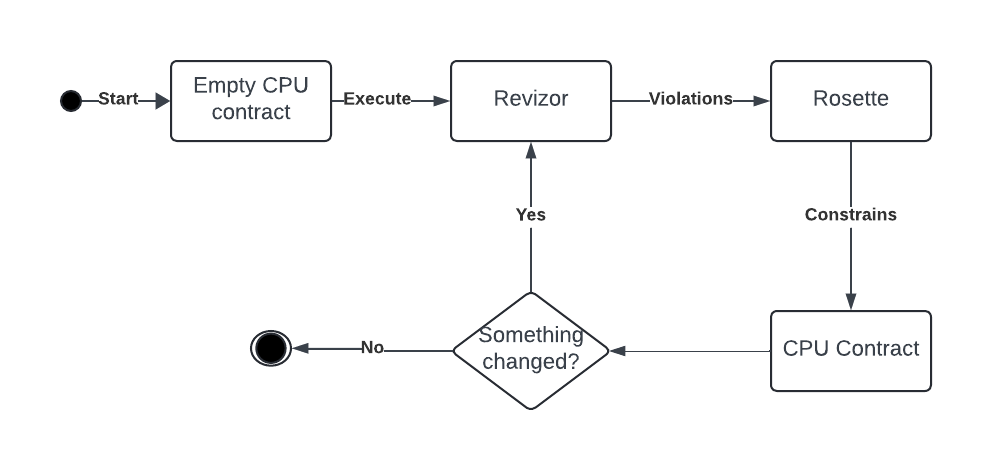
\includegraphics{images/Thesis.png}
  \end{center}
  \caption{Picture of the synthesis loop}
  \label{loop}
\end{figure}
\section{DSL}
\label{cha:DSL} To represent the CPU contract, the researchers needed a language
that was able to describe the ISA of a CPU and its contract. To archive this need,
at the beginning of the project, they developed a Domain Specific Language (DSL).
This language is able to define, check and evaluate a number of boolean conditions,
such as AND, OR, NOT, EQUAL, and to access CPU's registers. Here is a basic example
of a DSL code, that if a condition (that is always true in this case) is met, then
it traces the Program Counter (PC) register:

\begin{verbatim}
  (IF (BOOL #t) (REG 7)) # Register 7 is the PC
\end{verbatim}

This snippet is the most basic example of a CPU contract, that is used across the
project for testing purposes only.

The language was pretty easy to read and write, and did the job for the
bootstrapping of the project, and the first steps of research. This was enough
as a proof of concept to see whether the whole system was working, but now with the
further steps of the project, this is not enough anymore. To have a more research-validated,
robust, complete and universal language, the team decided to switch from this
DSL to using the BIR language (more in \cref{cha:BIR}), and the whys in the last
section of this \cref{cha:Language comparison}.

\section{BIR}
\label{cha:BIR} Binary Intermediate Representation (BIR, \cite{bir_pub}) is a
descriptive language developed by a group of researchers, that were trying to make
analysis of binary files, with the goal of validating them. To do so, they
needed a language that was platform independent, and that represented the ISA of
a CPU. The goal of the language is to be clear, meaning that it has only explicit
type changes, leaving no room for side effects and abstracted behaviors. BIR has
functionalities such as blocks, jump, assignment and so on. In our project, the part
of BIR that was used are the expressions. When we talk about expressions in BIR
we mean the following possible statements:
\begin{itemize}
  \item \textbf{Constant}: A constant value, in most cases a numeric value.

  \item \textbf{Unary operation}: Operation performed on a singular value, such
    as binary NOT, or change sign operation.

  \item \textbf{Binary expressions}: Operation performed on two values,
    combining them, such as SUM, MULT and so on. The operators need to be compatible
    with one another, meaning they need to have the same binary precision

  \item \textbf{Binary Predicates}: A function that returns a boolean value computing
    from two values. An example is the EQ predicate, checking equality of two given
    values.

  \item \textbf{Variable}: Usage of variables, such as the value inside a given
    register, abstracting from the value itself.

  \item \textbf{IfThenElse statement}: A conditional statement with a condition,
    and two branches that are evaluated and executed according to the condition
    itself.

  \item \textbf{Load}: Load a value from a given memory address.

  \item \textbf{Store}: Store a value in a given memory address.

  \item \textbf{OPERAND-VALUE}: Returns the value of the operand for a given operation
    code

  \item \textbf{OPERAND-TYPE}: Returns the type of the operand for a given operation
    code

  \item \textbf{OPERAND-ACCESS}: Returns the access mode of the operand for a given
    operation code

  \item \textbf{OPCODE}: Returns the opcode of the instruction that has just been
    executed

  \item \textbf{SLIDE}: Slide the bits of a given value, extracting a range of
    bits from it.
\end{itemize}

Following there is a simple example of each one of the possible expressions that
has been used in the project, with a brief comment on the meaning of them.
\begin{verbatim}
- (BExp_Const (bv 1 Bit32)) # Constant value 1, in binary vector of 32 bits.
- (BExp_UnaryExp (BIExp_ChangeSign (BExp_Const (bv 42 Bit8)))) # Change sign of 42
- (BExp_BinExp BIExp_Plus (BExp_Const (bv 12 Bit8)) (BExp_Const (bv 30 Bit8))) # Sum
of 12 and 30
- (BExp_BinPred BIExp_Equal (BExp_Const (bv 12 Bit8)) 
(BExp_Const (bv 30 Bit8))) # Check if 12 is equal to 30
- (BExp_Den (BVar REG 1)) # Value inside register R1
- (BExp_IfThenElse (BExp_BinPred BIExp_Equal (BExp_Const (bv 12 Bit8)) 
(BExp_Const (bv 30 Bit8))) (BExp_Const (bv 42 Bit8)) (BExp_Const (bv 50 Bit8))) 
# If 12 is equal to 30, return 42, else return 50
- (BExp_Load BExp_Den (BVar REG 1) (BExp_Const (bv 0 Bit32)) BEnd_LittleEndian Bit64) 
# Load value from memory address 0 in R1, in little endian, 64 bits
- (BExp_Store BExp_Den (BVar  REG 1) (BExp_Const (bv 0 Bit32)) BEnd_LittleEndian 
(BExp_Const(bv 2 Bit32))) # Store value 2 in memory address 0 in R1, in little endian
- (OPERAND-VALUE 1) # Return the value of the operand for the operation code 1
- (OPERAND-TYPE 1) # Return the type of the operand for the operation code 1
- (OPERAND-ACCESS 1) # Return the access mode of the operand for the operation code 1
- (OPCODE) # Return the opcode of the instruction that has just been executed
- (SLIDE 63 8 (OPERAND-VALUE 1)) # Used to extract a desired range of bits from a given address
\end{verbatim}

This range of expressions can also be nested and chained, to make more complex
constructs and represent more engineered ISAs, and for our purpose contracts.

\section{Language comparison}
\label{cha:Language comparison} Multiple reason concurred to the decision of switching
from the DSL to BIR. Some of them are technical, while some are more research-based.

Starting with the technical side, the DSL did not implement the majority of the
operations that a modern processor can perform, failing in representing completely
a CPU contract. This could have been a huge limitation, since all this project aims
to completely sinthesize a contract, and not having all the pieces to do so, would
have been a limitation, given the fact that vendors are using increasingly
complex contracts. As mentioned in \cref{cha:DSL}, the DSL was a good option for
the beginning and the proof of concept phase of the project, but could have never
been enough for the final goal of the project.

On the other hand, there is BIR. It is a language that, following modern CPU
architecture, is complete, and very explicit in its syntax. As we pointed out in
previous sections, while the DSL has a pretty simple syntax, BIR is more complex,
probably a bit harder to write, but way simpler and more clear to read. And
since almost no code for this project is going to be written by hand, this is a advantage
that BIR has. Also, the fact that BIR is complete makes it a better option, also
for future development, or current usage of the tool chain for more complex CPUs.

The DSL was also developed almost on the flight, for this specific project, while
BIR was created with the goal in mind to represent specifically and in a more general
fashion all CPU's ISA. BIR is therefore research-based, and engineered for the purpose
that we are aiming in this project. Even if this had never been the case, such a
lack of research in the DSL could have meant some limitations in the future, or
the need to change some parts of the code, slowing down further development.

BIR has also the feature that all his expressions are explicit and platform independent.
This means that once we write an IfThenElse statement in this language, the only
code that gets executed is that one, with no hidden behaviors or side effects, while
this was not explicitly the case for the DSL.

One last technical reason that played a major role in the choice, is the fact
that BIR's syntax is pretty close to a lot of dialects used in other security-related
tools. One good example is the Valgrind IR, \cite{valgrind}, a framework used for
dynamic analysis and threading bugs. Such a cohesion with already existing state-of-the-art
tooling would make the barrier to entry lower for other interested researchers
or security experts in the usage of this tool.

The last reason was that the BIR language created by some researchers that are
part of the project, and this would have made the integration of the language in
the project easier, and further development easier. This was therefore also a need
of the team, and not only a set of technical reasons. Having all the parties aligned
on the same language, meant more stability and long term maintainability of the
project.

This is why, in the end, the team decided to pursue the migration.